% !TeX spellcheck = es_MX-SpanishMexico
%----------------------------------------------------------------------------------------------------
%                           		  ENTRE LÍNEAS DE TIERRA

% Curso: Arqueología Bíblica
% Módulo 1: Introducción, Definiciones y Conceptos
% Elabora: Rodrigo Gerardo Trejo Arriaga

%----------------------------------------------------------------------------------------------------

% FORMATO DEL DOCUMENTO


\documentclass[11pt]{article} % Letra estandar

\usepackage[utf8]{inputenc}

%\usepackage{tgadventor}
%\renewcommand{\familydefault}{\sfdefault}

\usepackage[light,math]{iwona}

\usepackage[T1]{fontenc}


\usepackage[spanish]{babel}
\addto\captionsspanish{\renewcommand{\abstractname}{\large{Introducción}}}

\usepackage[margin=1in,letterpaper]{geometry}

\usepackage{fancyhdr} % Paquete para personalizar encabezado y pie de página
\pagestyle{fancy} % Establece que personalizaremos el pie de pagina y el encabezado
\setlength{\headheight}{13.59999pt} % Establece la altura del encabezado
\fancyhead[R]{\textcolor{darkBlue}{Teoría de la Computación}} % Encabezado derecho
\fancyhead[L]{\textit{\textcolor{darkBlue}{Escuela Superior de Cómputo}}} % Encabezado izquierdo
\fancyfoot[L]{\textit{\textcolor{darkBlue}{Práctica 6}}} % Pie de página izquierdo 
\fancyfoot[R]{\textcolor{darkBlue}{\thepage}} % Pie de página  derecho
\fancyfoot[C]{} % Elimina la nueración central de páginas en el pie de página
\renewcommand{\headrulewidth}{0.5pt} % Grosor de la linea de encabezado
\renewcommand{\footrulewidth}{0.5pt} % Grosor de la linea de pie de página

\usepackage{enumitem}

\usepackage{changepage}

\usepackage{graphicx}

\usepackage{tabularx}

\setlength{\parskip}{8pt}

\usepackage{xcolor}
\definecolor{darkBlue}{rgb}{0,0,0.31}
%\definecolor{darkBlue}{rgb}{0,0,0.5}
\definecolor{munsell}{rgb}{0.0, 0.5, 0.69}
\definecolor{indigo}{rgb}{0.0, 0.25, 0.42}
\renewcommand{\footrulewidth}{2pt}
\renewcommand{\footrule}{\hbox to\headwidth{\color{darkBlue}\leaders\hrule height \footrulewidth\hfill}}

\usepackage{colortbl}

\usepackage{titlesec}
\titleformat{\section}
{\normalfont\Large\bfseries\color{darkBlue}}{\thesection.}{1em}{}

\usepackage{tabularx}

\usepackage{textcomp}

\usepackage{titling}

\usepackage{apacite}

\usepackage{amsmath}
\bibliographystyle{apacite}

%\usepackage{natbib}
%\setlength{\bibsep}{6pt}

\usepackage{setspace}

\usepackage{listings}


% Define tus propios colores en tonos de azul
\definecolor{codeblue}{rgb}{0.25,0.5,0.5}
\definecolor{backcolour}{rgb}{0.95,0.95,0.92}
\definecolor{commentblue}{rgb}{0.3,0.3,0.6}
\definecolor{keywordblue}{rgb}{0.2,0.2,0.7}
\definecolor{stringblue}{rgb}{0.15,0.2,0.9}

\lstdefinestyle{bluepythonstyle}{
	language=Python,
	basicstyle=\ttfamily\small,
	commentstyle=\color{commentblue},
	keywordstyle=\color{keywordblue},
	numberstyle=\tiny\color{codeblue},
	stringstyle=\color{stringblue},
	backgroundcolor=\color{backcolour},
	breaklines=true,
	captionpos=b,
	abovecaptionskip=1\baselineskip,
	showstringspaces=false,
	frame=lines,
	numbers=left,
	xleftmargin=\parindent,
	tabsize=4
}
\lstset{style=bluepythonstyle}



\renewcommand{\thesection}{\Roman{section}}

%----------------------------------------------------------------------------------------------------
% CUERPO DEL DOCUMENTO

\begin{document}
	
	\begin{titlepage}
		\centering
		{
\includegraphics[width=0.25\textwidth]{descarga}\par}
		\vspace{0.5cm}
		{\bfseries\huge Escuela Superior de Cómputo \par}
		\vspace{0.7cm}
		{\scshape\LARGE Teoría de la Computación \par}
		\vspace{0.3cm}
		\vspace{3.1cm}
		{\scshape \Huge \textbf{Práctica 6:}  \par}
		\vspace{0.03cm}
		{{\LARGE \textit{AUTÓMATA DE PILA}} \par}
		%\vfill
		\vspace{3.5cm}
		{\Large Autor: \par}
		{\Large Rodrigo Gerardo Trejo Arriaga \par}
		%\vfill
		\vspace{3cm}
		{\Large Diciembre 2023 \par}
	\end{titlepage}
	
	\begin{center}
		\vspace*{0.1cm}
		{\huge \textcolor{darkBlue}{\textbf{Práctica 6:}} \par}
		
		{\Large \textcolor{darkBlue}{\textbf{\textit{AUTÓMATA DE PILA}}}}
	\end{center}
	
	
	\section{Introducción}
	Los autómatas de pila son un tipo de autómata abstracto que puede ser visto como una extensión de los autómatas finitos. Son particularmente útiles para el análisis de ciertos tipos de lenguajes formales como los lenguajes libres de contexto. Un autómata de pila hace uso de una pila para mantener un historial de información que le permite realizar transiciones que dependen no solo del estado actual y la entrada, sino también del contenido de la pila [1].
	
	\section{Definición Formal [2]}
	Un autómata de pila se define como una 6-tupla $(Q, \Sigma, \Gamma, \delta, q_0, F)$ donde:
	\begin{itemize}
		\item $Q$ es un conjunto finito de estados.
		\item $\Sigma$ es un conjunto finito de símbolos de entrada, conocido como el alfabeto de entrada.
		\item $\Gamma$ es un conjunto finito de símbolos de pila.
		\item $\delta: Q \times (\Sigma \cup \{\epsilon\}) \times \Gamma \rightarrow \mathcal{P}(Q \times \Gamma^*)$ es la función de transición.
		\item $q_0 \in Q$ es el estado inicial.
		\item $F \subseteq Q$ es el conjunto de estados de aceptación.
	\end{itemize}
	
	\section{Funcionamiento}
	El funcionamiento de un autómata de pila se basa en su capacidad para leer símbolos de entrada y manipular la pila según la función de transición $\delta$. En cada paso, el autómata [2]:
	\begin{enumerate}
		\item Observa el símbolo actual de la entrada y el símbolo en la cima de la pila.
		\item Realiza una transición a un nuevo estado y modifica la pila según $\delta$.
		\item Puede leer el siguiente símbolo de entrada o repetir el paso con el mismo símbolo.
	\end{enumerate}
	
	\section{Ejemplo}
	Consideremos un autómata de pila simple que reconoce el lenguaje $\{ a^n b^n | n \geq 0 \}$. La idea es usar la pila para contar el número de $a$s y luego verificar que hay un número igual de $b$s.
	
	\section{Instrucciones}
	
	El programa diseñado debe cumplir con las siguientes especificaciones:
	
	\subsection{Entrada de la Cadena}
	\begin{itemize}
		\item La cadena a evaluar puede ser ingresada por el usuario o generada automáticamente.
		\item En caso de generación automática, la longitud de la cadena no debe exceder los 100,000 caracteres.
	\end{itemize}
	
	\subsection{Evaluación del Autómata}
	\begin{itemize}
		\item El programa debe mostrar la evaluación del autómata a través de descripciones instantáneas (IDs).
		\item Esta evaluación debe ser mostrada tanto en pantalla como guardada en un archivo.
	\end{itemize}
	
	\subsection{Animación del Autómata}
	\begin{itemize}
		\item El autómata de pila debe ser animado si la longitud de la cadena es menor o igual a 10 caracteres.
	\end{itemize}
	
	
	
	\section{Resultados}
	
	
	\begin{figure}[h]
		\centering
		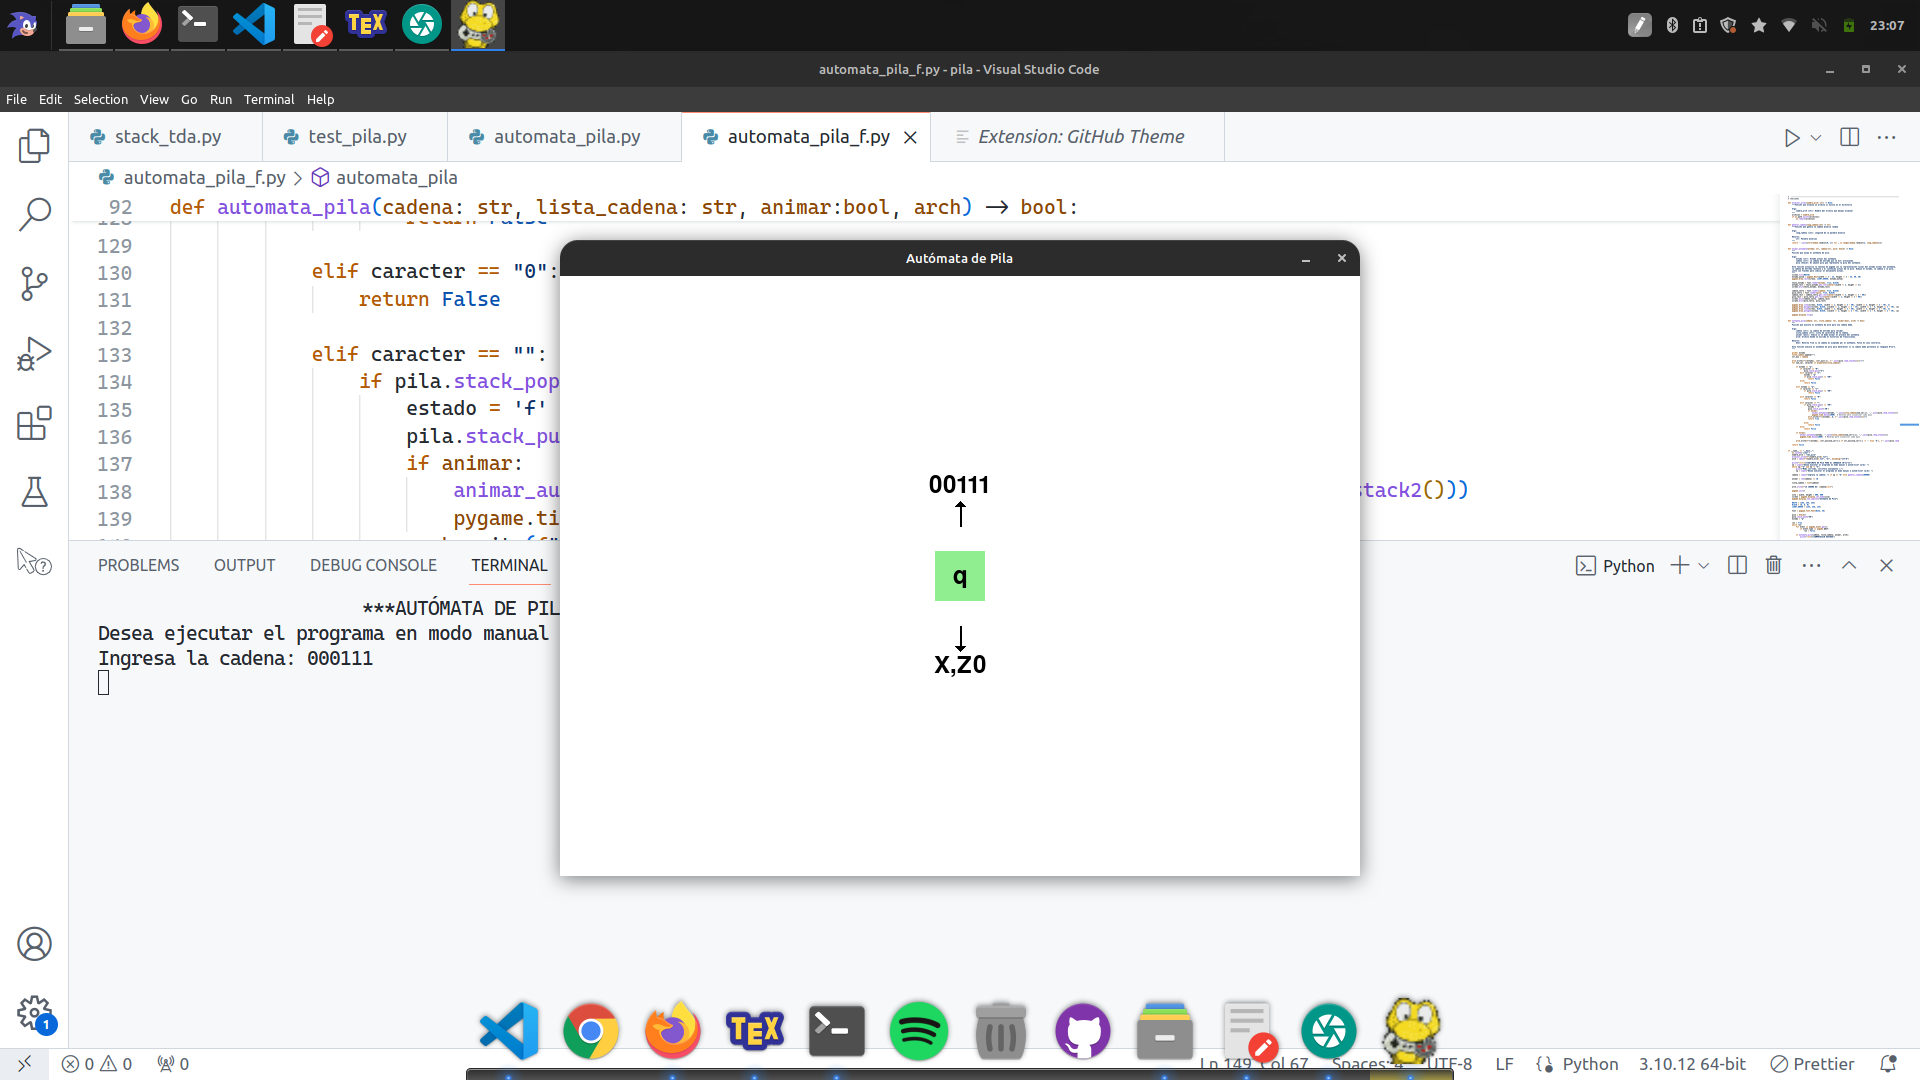
\includegraphics[width=0.9\textwidth]{manual}
		\caption{Modo manual - Animación de la pila}
	\end{figure}
	
	\newpage
	
	
	\begin{figure}[h]
		\centering
		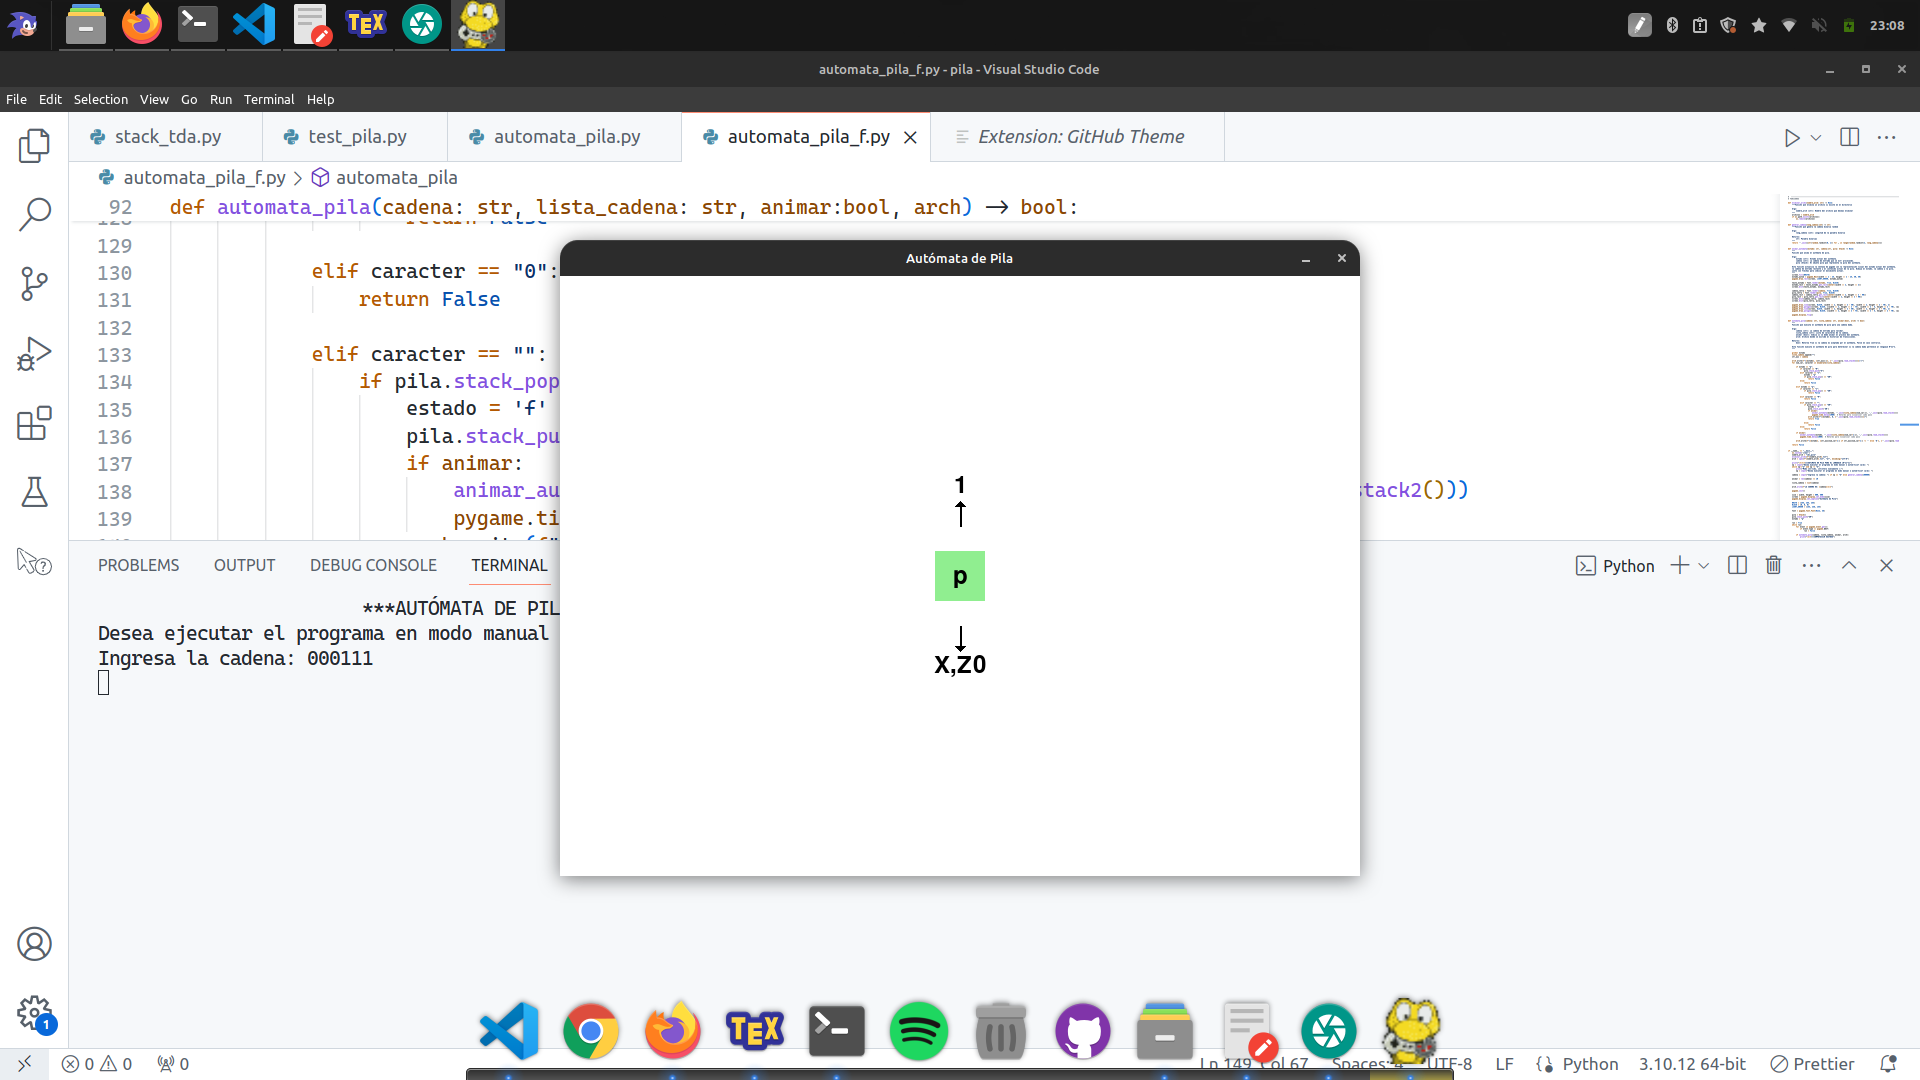
\includegraphics[width=0.8\textwidth]{manual2}
		\caption{Modo manual - Animación de la pila}
	\end{figure}
	
	\begin{figure}[h]
		\centering
		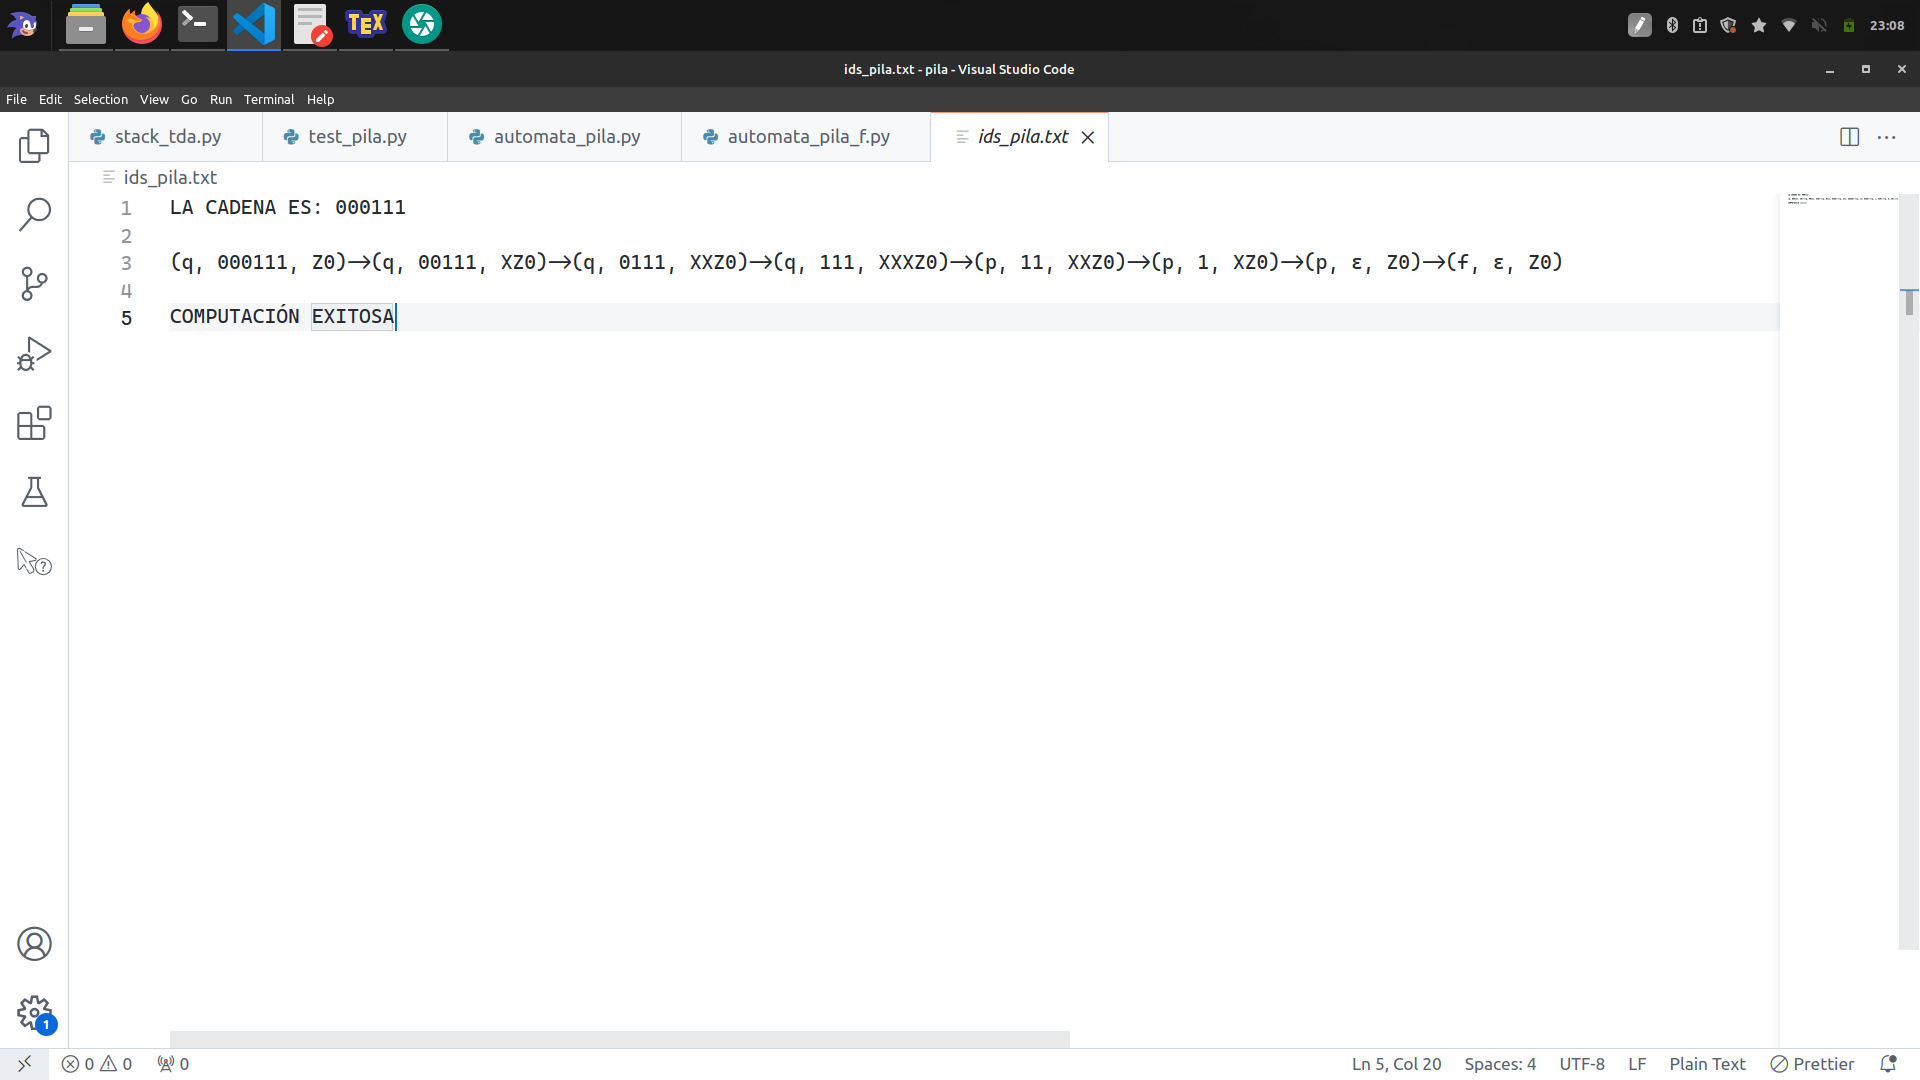
\includegraphics[width=0.8\textwidth]{arch1}
		\caption{Archivo del modo manual}
	\end{figure}
	
	\newpage
	
	\begin{figure}[h]
		\centering
		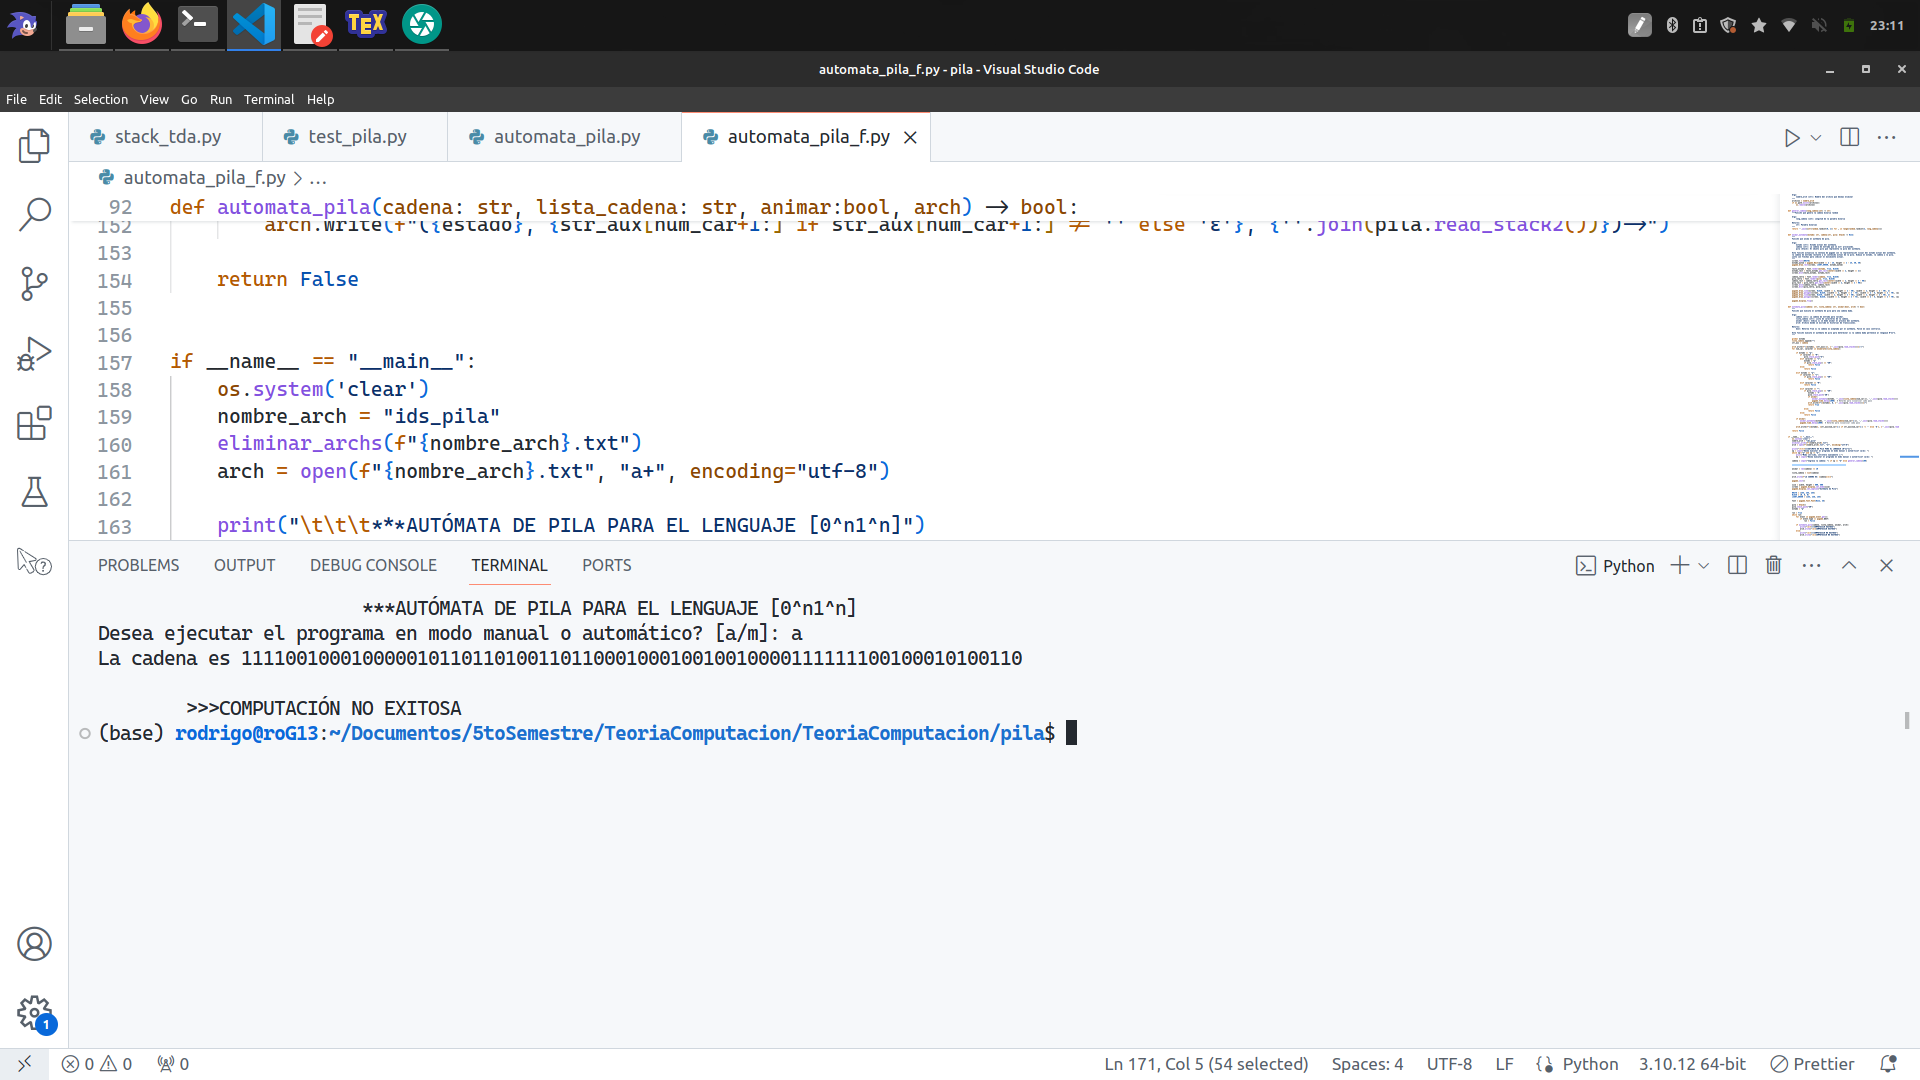
\includegraphics[width=0.8\textwidth]{auto}
		\caption{Modo automático}
	\end{figure}
	
	\begin{figure}[h]
		\centering
		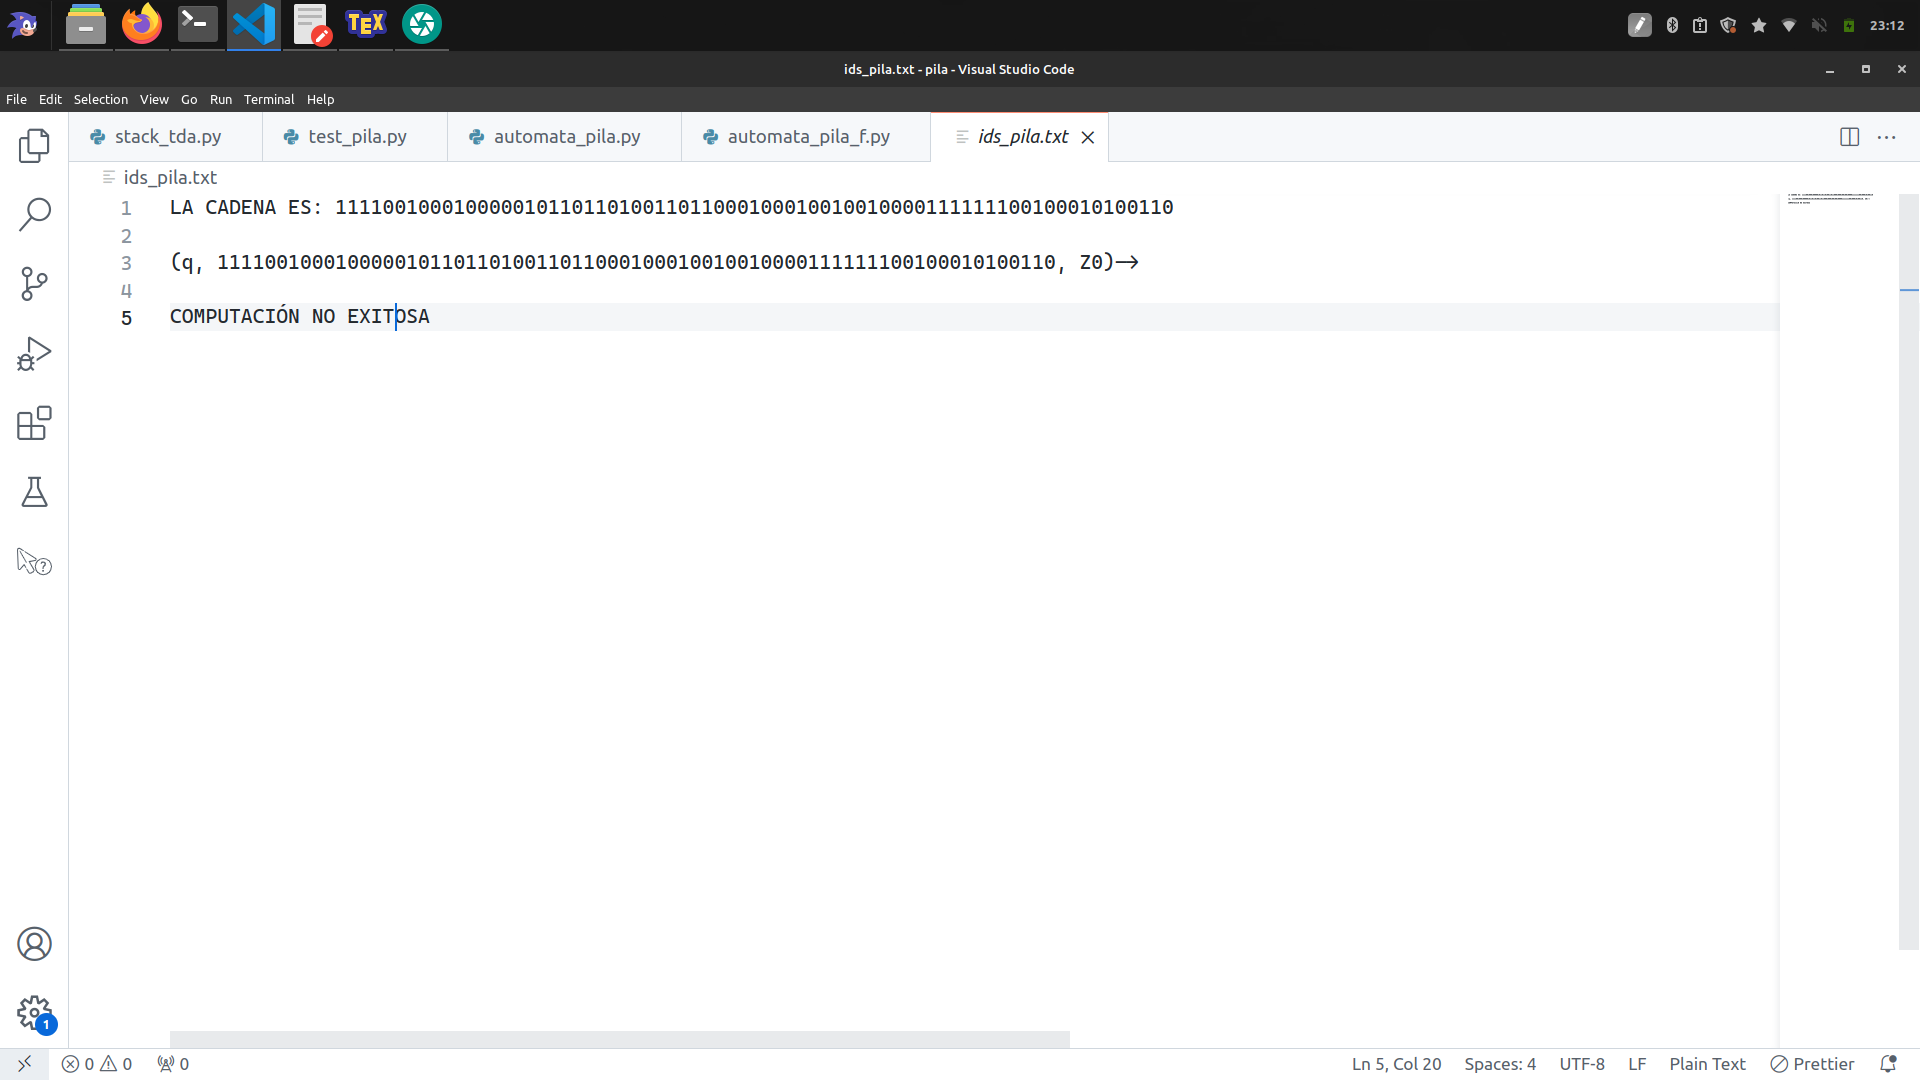
\includegraphics[width=0.8\textwidth]{arch2}
		\caption{Archivo del modo automático}
	\end{figure}
	
	\newpage
	\section*{Conclusión}
	La práctica con autómatas de pila ha proporcionado una comprensión profunda de su importancia en la teoría de la computación y su aplicación en el análisis de lenguajes libres de contexto. A través de la implementación de un autómata de pila que valida cadenas en el lenguaje específico $0^n1^n$, hemos podido observar de primera mano cómo estos modelos teóricos pueden ser transformados en herramientas de software efectivas.
	
	Esta práctica ha demostrado que, aunque los autómatas de pila son conceptualmente más complejos que los autómatas finitos, su capacidad para manejar una memoria auxiliar en forma de pila les permite reconocer patrones y estructuras que van más allá de las capacidades de los autómatas finitos. En particular, la habilidad para equilibrar y comparar segmentos de una cadena basándose en su longitud y contenido es fundamental en el análisis sintáctico en compiladores y en el procesamiento del lenguaje natural.
	
	
	De esta manera, esta práctica ha reforzado la relevancia de los autómatas de pila en la computación teórica y su aplicabilidad en problemas del mundo real, proveyendo una base sólida para futuras exploraciones en el campo de la teoría de la computación y el diseño de lenguajes de programación.
	
	\section*{Bibliografía}
	
	
	[1] Wikipedia. “Autómata con pila - Wikipedia, la enciclopedia libre”. Wikipedia, la enciclopedia libre. Accedido el 23 de diciembre de 2023. [En línea]. Disponible: https://es.wikipedia.org/wiki/Autómata\_con\_pila
	
	
	[2] “Automata de pila”. Lenguajes Formales y Autómatas. Accedido el 23 de diciembre de 2023. [En línea]. Disponible: https://ivanvladimir.gitlab.io/lfya\_book/docs/06dependedelcontexto/03autómatadepila
	deterministico/
	
	
	\newpage
	\section{Anexo - Código de Implementación}
	
	\begin{lstlisting}
	
		'''
		INSTITUTO POLITECNICO NACIONAL
		ESCUELA SUPERIOR DE COMPUTO
		
		INGENIERIA EN INTELIGENCIA ARTIFICIAL
		
		TEORIA DE LA COMPUTACION
		AUTOMATA DE PILA
		
		GRUPO: 5BM1
		ALUMNO: TREJO ARRIAGA RODRIGO GERARDO
		
		ESTE PROGRAMA GENERA UN AUTOMATA DE PILA QUE VALIDA SI UNA CADENA PERTENECE AL LENGUAJE 0^n1^n Y:
		i) SOLICITA AL USUARIO UNA CADENA A VALIDAR O LA GENERA DE MANERA RANDOM
		ii) ANIMA EL AUTOMATA DE PILA SI LA LONGITUD DE LA PALABRA ES MENOR A 10
		iii) GENERA LA HISTORIA DE ID's EN UN ARCHIVO DE TEXTO
		
		ULTIMA MODIFICACION: 23/12/2023
		'''
		
		#  --------------------------------------------------------------------------------------------------------------------
		# MODULOS Y LIBRERIAS IMPORTADAS
		
		import pygame
		import sys
		from stack_tda import Stack
		import os
		import random
		
		#  --------------------------------------------------------------------------------------------------------------------
		# FUNCIONES
		
		def eliminar_archs(nombre_arch: str) -> None:
			"""Funcion que elimina un archivo si existe en el directorio
			
			Args:
			nombre_arch (str): Nombre del archivo que deseas eliminar
			"""
			archivo1 = nombre_arch
			if os.path.exists(archivo1):
			os.remove(archivo1)
		
		
		def generar_cadena(long_cadena:int) -> str:
			"""Funcion que genera la cadena binaria random
			
			Args:
			long_cadena (int): Longitud de la palabra binaria
			
			Returns:
			str: Palabra binarias
			"""
			return ''.join([str(random.randint(0, 1)) for _ in range(random.randint(2, long_cadena))])
			
			
			def animar_automata(estado: str, cadena:str, pila: Stack) -> None:
			"""
			Funcion que anima el automata de pila.
			
			Args:
			estado (str): Estado actual del automata.
			cadena (str): La cadena de entrada que se esta procesando.
			pila (Stack): El objeto pila que representa la pila del automata.
			
			Esta funcion actualiza la ventana de pygame con la representacion visual del estado actual del automata, 
			la cadena de entrada restante y el contenido actual de la pila. Dibuja el estado, la cadena y la pila, 
			junto con flechas para indicar el movimiento actual.
			"""
			screen.fill(WHITE)
			estado_autom = pygame.Rect(width // 2 - 25, height // 2 - 25, 50, 50)
			pygame.draw.rect(screen, LIGHT_GREEN, estado_autom)
			
			texto_estado = font.render(estado, True, BLACK)
			estado_rect = texto_estado.get_rect(center=(width // 2, height // 2))
			screen.blit(texto_estado, estado_rect)
			
			cadena_letra = font.render(cadena, True, BLACK)
			pila_letra = font.render(pila, True, BLACK)
			cadena_rect = cadena_letra.get_rect(center=(width // 2, height // 2 - 90))
			pila_rect = pila_letra.get_rect(center=(width // 2, height // 2 + 90))
			screen.blit(cadena_letra, cadena_rect)
			screen.blit(pila_letra, pila_rect)
			
			pygame.draw.line(screen, BLACK, (width // 2, height // 2 - 50), (width // 2, height // 2 - 70), 2)
			pygame.draw.polygon(screen, BLACK, [(width // 2, height // 2 - 75), (width // 2 - 5, height // 2 - 70), (width // 2 + 5, height // 2 - 70)])
			pygame.draw.line(screen, BLACK, (width // 2, height // 2 + 50), (width // 2, height // 2 + 70), 2)
			pygame.draw.polygon(screen, BLACK, [(width // 2, height // 2 + 75), (width // 2 - 5, height // 2 + 70), (width // 2 + 5, height // 2 + 70)])
			
			pygame.display.flip()
		
		
		def automata_pila(cadena: str, lista_cadena: str, animar:bool, arch) -> bool:
			"""
			Funcion que ejecuta el automata de pila para una cadena dada.
			
			Args:
			cadena (str): La cadena de entrada para validar.
			lista_cadena (str): Lista de caracteres de la cadena.
			animar (bool): Indica si se debe animar el proceso del automata.
			arch: Archivo donde se escribe el historial de transiciones.
			
			Returns:
			bool: Retorna True si la cadena es aceptada por el automata, False en caso contrario.
			
			Esta funcion ejecuta el automata de pila para determinar si la cadena dada pertenece al lenguaje 0^n1^n. 
			"""
			
			global estado
			lista_cadena.append("")
			str_aux = cadena
			
			arch.write(f"({estado}, {str_aux[:]}, {''.join(pila.read_stack2())})->")
			for num_car, caracter in enumerate(lista_cadena):
			
			if estado == "q":
			if caracter == "0":
			pila.stack_push("X")
			elif caracter == "1":
			estado = "p"
			if pila.stack_pop() == "Z0":
			return False
			else:
			return False
			
			elif estado == "p":
			if caracter == "1":
			if pila.stack_pop() == "Z0":
			return False
			
			elif caracter == "0":
			return False
			
			elif caracter == "":
			if pila.stack_pop() == "Z0":
			estado = 'f'
			pila.stack_push('Z0')
			if animar:
			animar_automata(estado, ''.join(lista_cadena[num_car:]), ','.join(pila.read_stack2()))
			pygame.time.delay(1000)  # Retardo para visualizar cada paso
			arch.write(f"({estado}, e, {''.join(pila.read_stack2())})")
			return True
			
			else:
			return False
			else:
			return False
			
			if animar:
			animar_automata(estado, ''.join(lista_cadena[num_car+1:]), ','.join(pila.read_stack2()))
			pygame.time.delay(1000)  # Retardo para visualizar cada paso
			
			arch.write(f"({estado}, {str_aux[num_car+1:] if str_aux[num_car+1:] != '' else 'e'}, {''.join(pila.read_stack2())})->")
			
			return False
		
		
		if __name__ == "__main__":
			os.system('clear')
			nombre_arch = "ids_pila"
			eliminar_archs(f"{nombre_arch}.txt")
			arch = open(f"{nombre_arch}.txt", "a+", encoding="utf-8")
			
			print("\t\t\t***AUTOMATA DE PILA PARA EL LENGUAJE [0^n1^n]")
			op = input("Desea ejecutar el programa en modo manual o automatico? [a/m]: ")
			while op!="a" and op != "m":
			print("Modo invalido, intentelo nuevamente ):")
			op = input("Desea ejecutar el programa en modo manual o automatico? [a/m]: ")
			
			cadena = input("Ingresa la cadena: ") if op == "m" else generar_cadena(100000)
			
			print(f"La cadena es {cadena}") if op == "a" else None
			
			animar = len(cadena) <= 10
			
			lista_cadena = list(cadena)
			
			arch.write(f"LA CADENA ES: {cadena}\n\n")
			
			pygame.init()
			
			size = width, height = 800, 600
			screen = pygame.display.set_mode(size)
			pygame.display.set_caption("Automata de Pila")
			
			WHITE = (255, 255, 255)
			BLACK = (0, 0, 0)
			LIGHT_GREEN = (144, 238, 144)
			
			font = pygame.font.Font(None, 36)
			
			pila = Stack()
			pila.stack_push("Z0")
			estado = "q"
			
			run = True
			while run:
			for event in pygame.event.get():
			if event.type == pygame.QUIT:
			run = False
			
			if automata_pila(cadena, lista_cadena, animar, arch):
			print("\n\t>>>COMPUTACION EXITOSA")
			arch.write("\n\nCOMPUTACION EXITOSA")
			else:
			print("\n\t>>>COMPUTACION NO EXITOSA")
			arch.write("\n\nCOMPUTACION NO EXITOSA")
			
			run = False
			
			pygame.quit()
			sys.exit()
		
	
	
	\end{lstlisting}

	
	
\end{document}